%
% Template for DAS course projects
%
\documentclass[a4paper,11pt,oneside]{book}
\usepackage[latin1]{inputenc}
\usepackage[english]{babel}
\usepackage{amsfonts}
\usepackage{amsmath}
\usepackage{amssymb,amsmath,color}
\usepackage{graphicx}
\graphicspath{{./figs/}}
\usepackage{subcaption}
\usepackage{float}
\usepackage{tikz}
\usepackage{listofitems} % for \readlist to create arrays
\usepackage[outline]{contour} %
\usepackage{xcolor}

\babelhyphenation{con-nec-tions}
\babelhyphenation{com-pu-ta-tions}
\babelhyphenation{im-por-tant}
\babelhyphenation{track-ing}
\babelhyphenation{com-mu-ni-ca-tion}
\babelhyphenation{com-po-nent}
\babelhyphenation{dis-tri-bu-ted}
\babelhyphenation{de-vi-ces}

\tikzstyle{node}=[thick,circle,draw=blue,minimum size=22,inner sep=0.5,outer sep=0.6]
\tikzstyle{bias}=[thick,square,draw=black,minimum size=22,inner sep=0.5,outer sep=0.6]
\tikzstyle{node in}=[node,green!20!black,draw=green!30!black,fill=green!25]
\tikzstyle{node hidden}=[node,blue!20!black,draw=blue!30!black,fill=blue!20]
\tikzstyle{node out}=[node,red!20!black,draw=red!30!black,fill=red!20]
\tikzstyle{connect}=[thick,black] 
\tikzset{ % node styles
  node 1/.style={node in},
  node 2/.style={node hidden},
  node 3/.style={node out},
}
\def\nstyle{int(\lay<\Nnodlen?min(2,\lay):3)} % map layer number onto 1, 2, or 3

\usepackage{hyperref}
\hypersetup{
    colorlinks,
    citecolor=black,
    filecolor=black,
    linkcolor=blue,
    urlcolor=black
}


\begin{document}
\pagestyle{myheadings}

%%%%%%%%%%% Cover %%%%%%%%%%%
\thispagestyle{empty}                                                 
\begin{center}                                                            
    \vspace{5mm}
    {\LARGE UNIVERSIT\`A DI BOLOGNA} \\                       
      \vspace{5mm}
\end{center}
\begin{center}
  
\includegraphics[scale=.27]{logo_unibo}
\end{center}
\begin{center}
      \vspace{5mm}
      {\LARGE School of Engineering} \\
        \vspace{3mm}
      {\Large Master Degree in Automation Engineering} \\
      \vspace{20mm}
      {\LARGE Distributed Autonomous Systems} \\
      \vspace{5mm}{\Large\textbf{DISTRIBUTED CLASSIFICATION VIA NEURAL NETWORKS AND FORMATION CONTROL}}                  
      \vspace{15mm}
\end{center}
\begin{flushleft}                                                                              
     {\large Professors:}\\
     \textbf{\@ Giuseppe Notarstefano} \\
     \textbf{\@ Ivano Notarnicola} \\        
     \vspace{4mm}
	
	{\large Tutor:}\\
	\textbf{\@ Lorenzo Pichierri} \\
     \vspace{8mm}
\end{flushleft}
\begin{flushright}
      {\large Students:}\\
      {Simone Cenerini} \\
      {Giulia Cutini} \\
      {Riccardo Paolini} \\
\end{flushright}        %capoverso allineato a destra
\begin{center}
\vfill
      {\large Academic year \@2022/2023} \\
\end{center}



\newpage
\thispagestyle{empty}

%%%%%%%%%%% Abstract %%%%%%%%%%%%
\begin{center}
\chapter*{}
\thispagestyle{empty}
{\Huge \textbf{Abstract}}\\
\vspace{15mm}
\end{center}

The report shows the development of two projects that aim to present some of the possible applications of distributed systems in different fields.

\bigskip
The report is organized as follows: in the first chapter we describe the distributed implementation of a binary supervised classification task for images of handwritten digits. The aim is to run in parallel several neural networks by different agents that communicate only locally with neighbors, and thanks to a distributed algorithm, the \textit{Gradient Tracking algorithm} we expect them to obtain the same performances on a common test set. We show different tests we have performed, such as how the accuracy changes by changing the target digit or how the type of connection graph among agents influences the number of updates required to reach consensus.

\bigskip
In the second chapter we describe a ROS2 implementation of the distance-based formation control law by exploiting several real possible scenarios. The first test was to obtain different chosen shapes, as a formation for our team of robots, both in 2D and in 3D. 
Then we have introduced collision avoidance among the agents and tried to steer the formation according to a certain assigned motion or toward a target position. In order to do that, we have defined proper control laws to give to the leaders of the formation the required input to accomplish the task.
The simulations showed by means of RViz.


\tableofcontents \thispagestyle{empty}
% \listoffigures\thispagestyle{empty}

%%%%%%%%%% Introduction %%%%%%%%%%
\newpage
\chapter*{Motivations} 
Distributed systems play a crucial role in today's connected world where we need efficient and scalable solutions. Our project is motivated by the need to address complex challenges in machine learning and robotics through the power of distributed systems, in which agents aim at cooperatively solving complex tasks by local computation and communication.

\bigskip
The primary motivation behind our work is to leverage the collective computational resources of multiple agents to accelerate the training of neural networks. By dividing the work and doing tasks in parallel, our system helps the networks learn faster and reduces the time needed for training. This is especially useful when dealing with large amounts of data and complicated models that require a lot of computing resources.

In addition to enlarge computational capabilities, distributed systems offer inherent fault tolerance and resilience. Decentralizing computation and data storage reduces the risk of single points of failure, ensuring the system's robustness. This is crucial in critical applications.

Scalability is another key motivation for exploring distributed systems. As datasets grow exponentially, centralized systems often struggle to handle the increasing computational demands. Distributed systems can handle large amounts of data by easily adding more agents to the network, allowing efficient processing.

%\section*{Contributions}



%%%%%%%%%% Chapter Title %%%%%%%%%%
%%%%%%%%%% Chapter Title %%%%%%%%%%
\chapter{Distributed classification via Neural Network}

\begin{figure}
	\centering
	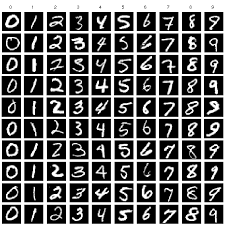
\includegraphics[scale=0.5]{mnist}
	\caption{Example of images from the \texttt{mnist} dataset}
	\label{mnist}
\end{figure}


In the first task we should classify a set of grayscale images. The \texttt{mnist} dataset, downloaded from the Keras library, collects images of handwritten digits of $28\times28$ pixels each one, with a value between 0 (black) and 255 (white), an example in figure \ref{mnist}. In order to perform our task we implemented a distributed classification where, given a predefined number of agents, each of them trains its own neural network. To make possible to the whole cyber-network to converge to a common value over the connection weights we have implemented a distributed Gradient Tracking algorithm. This approach ensures that consensus is reached even though these networks train only on locally available data, that is, they ''see'' only a fraction of the global optimization problem.

\section{Initial setup}
The first step was to prepare the dataset by reshaping and normalizing the images (file \texttt{lib/data\_load.py}). This is achieved by flattening the $28\times28$ pixel grayscale images in order to obtain a $[784,1]$ column vector, and normalizing the pixel intensities dividing them by a factor of $255$ in order to avoid a saturation of the activation function.

\bigskip
The classification problem we had to address is binary: we have to choose a digit (named as \texttt{target}) and assign the positive label ($1$) to the corresponding images, while, all the other images are labelled as negatives ($0$).
\begin{equation}
y_i = 
\begin{cases}
1, & \text{if label = \texttt{target}} \\
0, & \text{otherwise}
\end{cases}
\end{equation}

We have also performed a \textbf{balancing of the dataset} by sampling the same amount of images for each class ($50\%$ positives and $50\%$ negative), this makes the training more efficient and stable.

\section{Neural Network structure}

% NEURAL NETWORK SCHEME
\begin{figure}
\centering
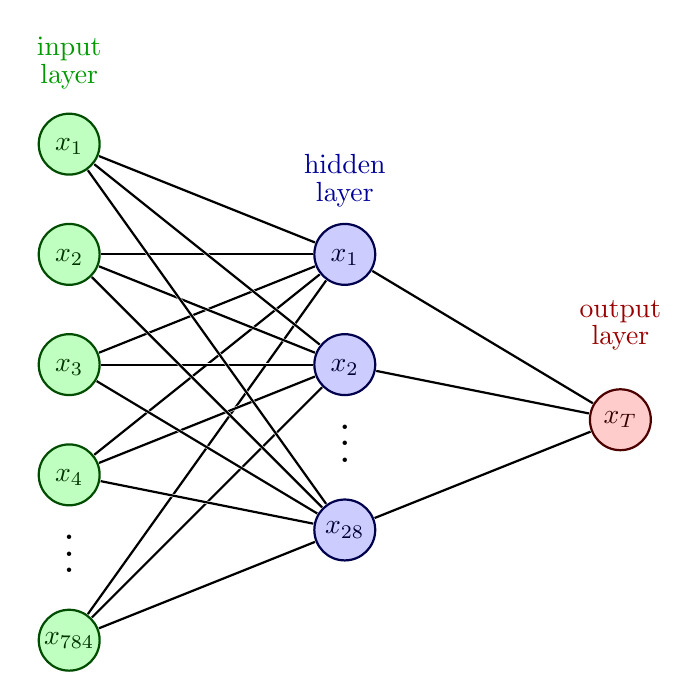
\begin{tikzpicture}[x=3.5cm,y=1.4cm]

\readlist\Nnod{5,3,1} % array of number of nodes per layer
\readlist\Nstr{n,m,k} 
\readlist\Cstr{\strut x,\strut x,{}} 
\def\yshift{0.5} % shift last node for dots


\foreachitem \N \in \Nnod{ 
\def\lay{\Ncnt} 
\pgfmathsetmacro\prev{int(\Ncnt-1)}
\message{\lay,}
\foreach \i [evaluate={\c=int(\i==\N); \y=\N/2-\i-\c*\yshift;
\index=(\i<\N?int(\i):"\Nstr[\lay]");
\x=\lay; \n=\nstyle;}] in {1,...,\N}{


% NODES
\ifnum\lay=1 % First Layer
  \ifnum\i=\N % Last neuron of first layer
    \node[node \n] (N\lay-\i) at (\x,\y) {$x_{784}$}; 
  \else
    \node[node \n] (N\lay-\i) at (\x,\y) {$\Cstr[\lay]_{\index}$};
  \fi
\fi

\ifnum\lay=2 % Second Layer
  \ifnum\i=\N % Last neuron of second layer
    \node[node \n] (N\lay-\i) at (\x,\y) {$x_{28}$}; 
  \else
    \node[node \n] (N\lay-\i) at (\x,\y) {$\Cstr[\lay]_{\index}$}; %empty
  \fi
\fi

\ifnum\lay=3 % Third Layer
  \node[node \n] (N\lay-\i) at (\x,\y) {$x_T$}; 
\fi


% CONNECTIONS
\ifnum\lay>1 % connect to previous layer
  \foreach \j in {1,...,\Nnod[\prev]}{ 
    \draw[connect,white,line width=1.2] (N\prev-\j) -- (N\lay-\i);
     \draw[connect] (N\prev-\j) -- (N\lay-\i);
}
\fi % nothing to connect first layer
      
}
\ifnum\lay<\Nnodlen % draw dots for all layers except the last one
    \path (N\lay-\N) --++ (0,1+\yshift) node[midway,scale=1.5] {$\vdots$};
    \fi
}

% LABELS
% \pixel[above=5,align=center,black] at (N1-1.90) {flatten\\[-0.2em]image}
  \node[above=5,align=center,green!60!black] at (N1-1.90) {input\\[-0.2em]layer};
  \node[above=2,align=center,blue!60!black] at (N2-1.90) {hidden \\[-0.2em]layer};
  \node[above=10,align=center,red!60!black] at (N\Nnodlen-1.90) {output\\[-0.2em]layer};
  
\end{tikzpicture}
\caption{Scheme of the neural network for image classification}
\label{NN_scheme}
\end{figure}


The structure of our neural network is conical, that is, the deeper layers contain fewer neurons than the earlier layers, it is drawn in figure \ref{NN_scheme}. 
The input layer is composed of $784$ neurons, equal to the dimension of the flattened input image. The hidden layer has only 28 neurons, as more neurons were not necessary for our task, but would simply increase the computational effort required. The last layer has just one neuron since we perform a binary classification, and thus only a number between $0$ and $1$ is required as a prediction.

With respect to the structure shown in figure \ref{NN_scheme} we have added the bias (a "fake" neuron with constant value always equal to 1) in the code implementation.

\bigskip
In this setting we obtain two sets of weights, one for the connections between the input and hidden layers, while the second one is for the connections between the hidden and output layers. In particular, each neuron of the generic layer $L^t$ is connected with all the neurons of the previous layer $L^{t-1}$ plus one connection for the bias, thus each set $W^t$ contains $|L^t| \cdot (|L^{t-1}| + 1)$ weights, where $W^t$ is the set of weights associated to the $t$ layer.

\bigskip
In a neural network, the activation function is the following mathematical function:
\begin{equation}
x_l^+= \sigma(x^T u_l + u_{l_0})
\end{equation}
with $\sigma: \mathbb{R} \to \mathbb{R}$.

Notation: $l$ identifies a neuron, a single computational unit, $u_l \in \mathbb{R}^{d+1}$ is the set of weights associated to it, with the bias ($u_{l_0}$), and $x$ is the "state" vector the neuron updates thanks to the activation function. 

\bigskip
The activation function introduces non-linearity to the neuron's output, allowing the network to learn and model complex relationships between inputs and outputs.

\bigskip
The activation function we used in this project is the \textbf{sigmoid} function (file \texttt{lib/network\_dynamics.py})
\begin{equation}
\sigma(\xi) = \frac{1}{1 + e^{-\xi}}
\end{equation}

where $\xi = x^T u_l + u_{l_0}.$

The derivative of the sigmoid function is:

\begin{equation}
\frac{d}{d\xi}\sigma(\xi) = \frac{\sigma(\xi)}{1 - \sigma(\xi)}
\end{equation}

The connections for our neural network have been randomly initialized according to a Gaussian distribution with zero mean and $0.01$ variance, the same for the bias.

\section{Training}
The training happens as a sequence of epochs, every epoch contains multiple minibatches that are small sets of images. For each mini-batch the computations are the following:

\begin{itemize}
    \item Forward pass to compute the prediction;
    \item Loss and gradient evaluation;
    \item Backward pass to compute the derivative of the loss function with respect to each weight of the network.
    \item Weights update.
\end{itemize}

The loss function we used is the \textbf{binary cross-entropy} 

\begin{equation}
J = - y \cdot \log(\hat{y}) - (1 - y) \cdot \log(1 - \hat{y})
\label{Cost_funct}
\end{equation}
where $\hat{y}$ is the prediction, i.e. the output value of the neuron of the output layer. These predictions are used to compute the gradient on the output layer and thus to start the backward pass on the network.

The derivative of the loss function, with respect to the prediction $\hat{y}$, is:

\begin{equation}
\frac{\partial J}{\partial \hat{y}} = - \frac{y}{\hat{y}} + \frac{1 - y}{1 - \hat{y}}
\end{equation}

\subsection{Gradient Tracking algorithm}

\begin{figure}[h]
	\centering
	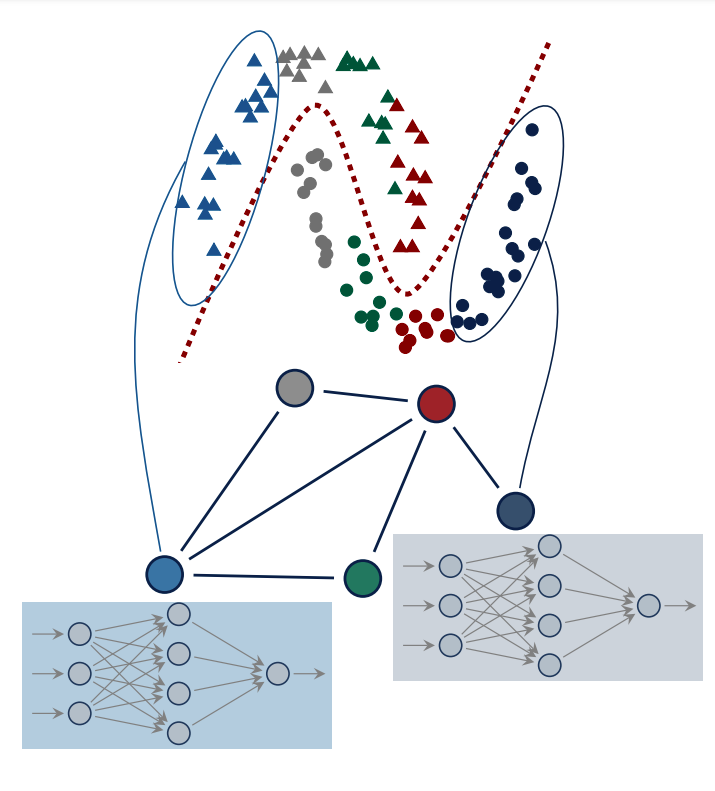
\includegraphics[scale=0.2]{Distributed_learning}
	\caption{Scheme of how distributed learning of neural networks works}
	\label{Distributed_learning}
\end{figure}

The training happens in a distributed fashion: several agents run a neural network with the same structure on different training sets and communicate with neighbors according to a certain communication graph. A scheme can be seen in figure \ref{Distributed_learning}

\bigskip
In a distributed computation, the communication topology is an important part of the problem. The communication between agents is modeled through a graph $G = (\{1, \ldots,N\}, E)$ where $N$ are the nodes (one for each agent) and $E$ are the edges. Since in our application we are working with undirected graphs, we can say than an agent $i$ can communicate with another agent $j$ if the the pair $(i,j) \in E$ or $(j,i) \in E$.

\bigskip
Thus, in agent's networks, the goal is to design a proper distributed algorithm, such as the \textbf{Gradient Tracking algorithm}, that allows multiple agents in the network to collectively solve an optimization problem by tracking the gradient information of a global objective function.
The optimization problem we need to solve is the following:
\begin{equation}
\min_{\textbf{u}} \sum_{i=1}^N J_i(\textbf{u})
\end{equation}
where $\textbf{u}$ is a common decision variable, while the cost function (expressed in formula \ref{Cost_funct}) is the sum of $N$ local contributes.

\bigskip
If we suppose that our optimization cost coupled problem has an optimal solution $\textbf{u}^*$, we want our optimization algorithm to make all agents update their own local estimates $\textbf{u}_i^k$ in such a way to converge to the optimal consensual value.

The formula of the algorithm are the following:
\begin {equation}
\begin{aligned}
u_i^{k+1} &= \sum_{j \in N_i} a_{ij} u_j^k - \alpha s_i^k, \quad & u_i^0 \in \mathbb{R}\\
s_i^{k+1}   &= \sum_{j \in N_i} a_{ij} s_j^k + \big( \nabla J_i(u_i^{k+1}) - \nabla J_i(u_i^k)\big) , \quad & s_i^0 = \nabla J_i(u_i^0) \\
\end{aligned}
\end{equation}
where the variable $s_i^k$ is a local estimate used as an estimation of the local descent direction, and $u_i^k$ is the local update of the connection weights. 

\bigskip
The assumptions required by the algorithm to converge are the following:
\begin{itemize}
\item \textit{Ass.1}: Let  $a_{ij}$, $i,j \in \{1, \ldots, N\}$ be non-negative entries of a weighted adjacency matrix A associated to the undirected and connected graph $G$, with $a_{ii}>0$ and A doubly stochastic.
\item \textit{Ass.2}: For all $i \in \{1, \ldots, N\}$ each cost function $f_i: \mathbb{R}^d \to \mathbb{R}$ satisfies the following conditions: strongly convex with coefficient $\mu >0$, and Lipschitz continuous gradient with constant $L>0$.
\end{itemize}
Thanks to these assumptions it can be shown that there exists a $\alpha^*>0$ (constant stepsize) such that for all $\alpha \in (0,\alpha^*)$, the sequence of local solution estimates $\{u_i^k\}_{k\geq0}$ asymptotically converge to a (consensual) solution $\textbf{u}^*$ of the problem.

\bigskip
The adjacency matrix $A$ from which we extract the coefficient $a_{ij}$ is, as previously said, a non-negative matrix such that the entry $(i,j)$ is $a_{ij}>0$ if $(i,j)$ is an edge of the graph, $a_{ij}=0$ otherwise.
In our implementation (file \texttt{lib/graph.py}) we choose the weights according to the \textit{Metropolis Hastings} rule:
\begin{equation}
A_{ij} = 
\begin{cases}
\frac{1}{\max\{d_i,d_j\}+1},  &\text{if } (i,j) \in E\, \text{and}\, i \neq j \\
1-\sum_{h \in N_i} A_{ih}, &\text{if }  i=j \\
0, &\text{otherwise}
\end{cases}
\end{equation}
where $d_i$ and $d_j$ are the out-degrees respectively of node $i$ and $j$.

\bigskip
In our implementation of the Gradient Tracking algorithm, applied to the federated learning of a neural network,  we compute the new weights $u^{k+1}$ before the forward pass, contrarily the auxiliary variable $s^{k+1}$ is obtained after the backward pass since its computation requires the gradient computed with the new weights $u^{k+1}$.

\section{Experiments and Results}
For testing the network we use the test set without splitting it, in this way we can check whether the agents provide equal results, given that they should reach consensus to the same weights. 

\bigskip
The performance are evaluated using accuracy as a metric. A threshold at value 0.5 is applied to the predictions as they are in the range $[0, 1]$.

\begin{equation}
\hat{y}_i = 
\begin{cases}
1, & \hat{y}_i > 0.5 \\
0, & \hat{y}_i \le 0.5
\end{cases}
\end{equation}
where $i$ indicates a single image, and $\hat{y}_i$ its prediction value.

\bigskip
A prediction is said to be correct if the label is equal to $\hat{y}$, incorrect otherwise.
The accuracy has been computed as the ratio between the number of correct predictions of an agent over the total number of tests.

\bigskip
We made different experiments to verify the functioning of the network both as the hyper-parameters such as step-size change but also as the target class or graph changes (file \texttt{lib/config.py}). The results are reported in the following.

\newpage
\section{First test: efficiency of the neural network}
In the first experiment we want to inspect the convergence of the network. In this configuration we have 5 agents communicating according to a \textit{cycle graph} \ref{cycle_graph}, each of them is trained on 32 mini-batches containing 8 samples each for a total of 256 images. 
We have trained our network over $5000$ epochs with a constant stepsize equal to $5e^{-4}$.

\begin{figure}[h]
    \centering
    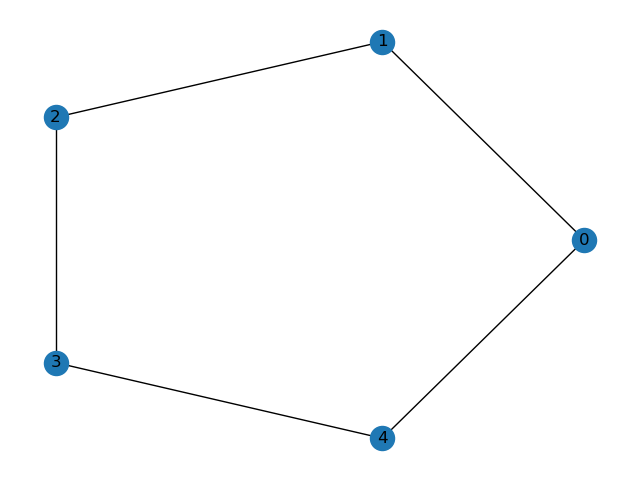
\includegraphics[width=0.32\textwidth]{cycle/graph}
    \caption{Communication graph}
    \label{cycle_graph}
\end{figure}

From the plots in \ref{cycle_cost_grad} we can appreciate the evolution of the cost function and the norm of the gradients, both on a logarithmic scale. We have decided to plot both the evolution of the mean values over the agents, and the single agent's values (dotted lines). In particular it is possible to observe that the magnitude of the gradients quickly decreases over the firsts epochs, and then slows down as the network improves.

\begin{figure}[h]
\centering
	\begin{subfigure}{0.49\textwidth}	
	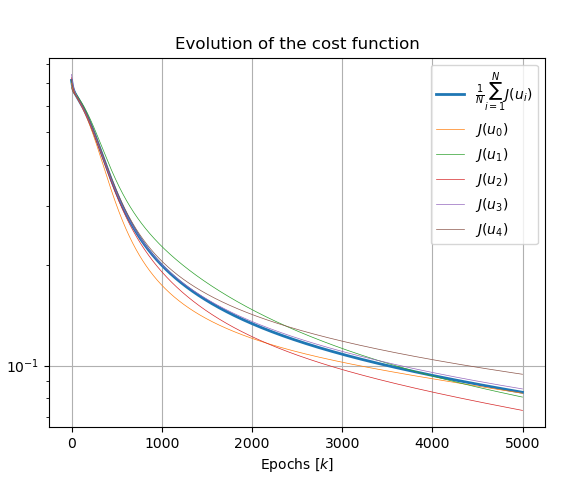
\includegraphics[width=\textwidth]{cycle/cost_log}
	\caption{Cost evolution in log-scale}
	\end{subfigure}
\hfill
	\begin{subfigure}{0.49\textwidth}	
	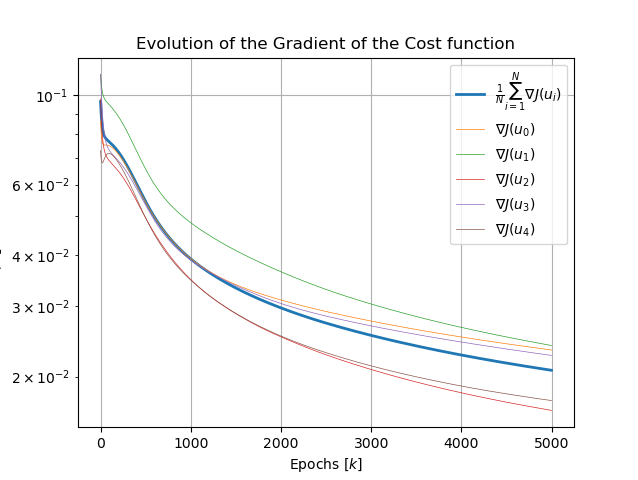
\includegraphics[width=1.08\textwidth]{cycle/gradient_log}
	\caption{Gradient evolution in log-scale}
	\end{subfigure}
\caption{Evolution of the cost function and the gradient.}
\label{cycle_cost_grad}
\end{figure}

\bigskip

After that, to check if the network reaches the consensus, we choose the weight associated to a single connection (in particular the one that connects the first neuron of the hidden layer with the neuron of the output layer, called $u_c$). We have decided to plot, in order to have a more readable graph, the difference between the value of this connection and its mean value across all the agents.
\begin{equation}
\text{Error} = u_{ci} - \frac{1}{N}\sum_{i=1}^N u_{ci}
\end{equation}
Theoretically, at consensus, this value should be equal to to zero. Indeed, from the plot \ref{cycle_consensus} we can see that this difference approaches the zero value, therefore the networks converge to a consensus.  These plots have been done over $3000$ updates, in fact, since we are working with the minibatches, each epoch corresponds to a number of updates equal to the number of a minibatches.

\bigskip
In this experiment, we reached an accuracy of $97.6\%$ on the test set.

\begin{figure}[h]
\centering
	\begin{subfigure}{0.49\textwidth}	
	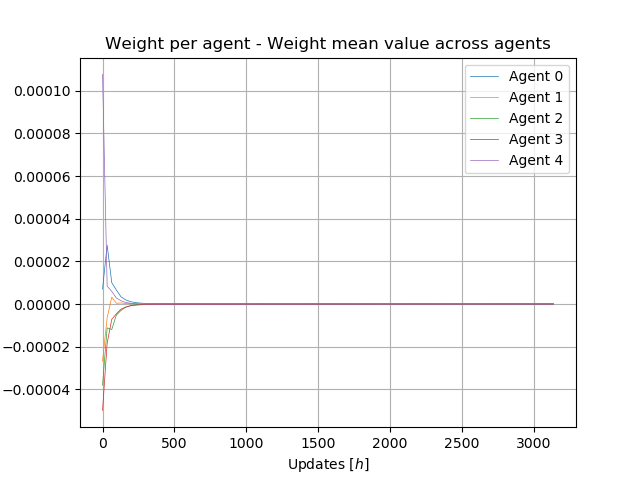
\includegraphics[width=\textwidth]{cycle/weight_100}
	\caption{Consensus error evolution}
	\end{subfigure}
\hfill
	\begin{subfigure}{0.49\textwidth}	
	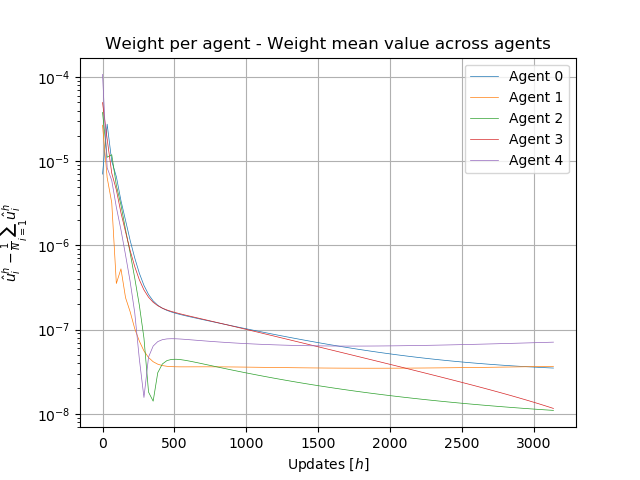
\includegraphics[width=\textwidth]{cycle/weight_100_log}
	\caption{Consensus error evolution in log-scale}
	\end{subfigure}
\caption{Consensus error evolution}
\label{cycle_consensus}
\end{figure}

\section{Second test: different digits}
In the second experiment, we check whether the target digit impacts the network behaviour, in particular we repeat the previous test for all the possible target digits. The following results are obtained over a reduced number of epochs in order to train the network in a quite short time and, as a consequence a bigger stepsize equal to $1e^{-2}$.

\begin{center}
\begin{tabular}{|c|c|}
\hline
Target digit & Accuracy \\
\hline
0 & 97.66\% \\
1 & 96.88\% \\
2 & 94.92\% \\
3 & 92.96\% \\
4 & 96.87\% \\
5 & 91.01\% \\
6 & 95.70\% \\
7 & 96.48\%\\
8 & 96.48\% \\
9 & 94.53\% \\
\hline
\end{tabular}
\end{center}

The table highlights how the simplest digit to be recognized is $0$ while the most difficult is $5$. Nevertheless the accuracy obtained are very good in all the several simulations.

\section{Third test: impact of graph shape on consensus}
In the last test, we checked the impact of the shape of the communication graph on the epochs required to reach consensus.

\begin{figure}[H]
\centering
    \begin{subfigure}{0.32\textwidth}
    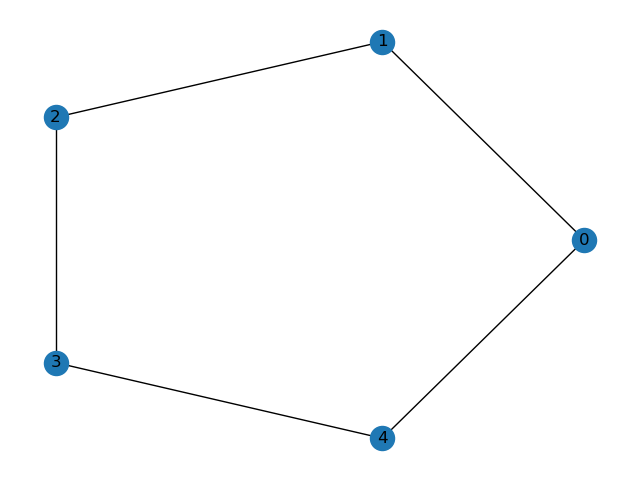
\includegraphics[width=\textwidth]{cycle/graph}
    \caption{Cycle graph}
    \end{subfigure}
\hfill
    \begin{subfigure}{0.32\textwidth}
    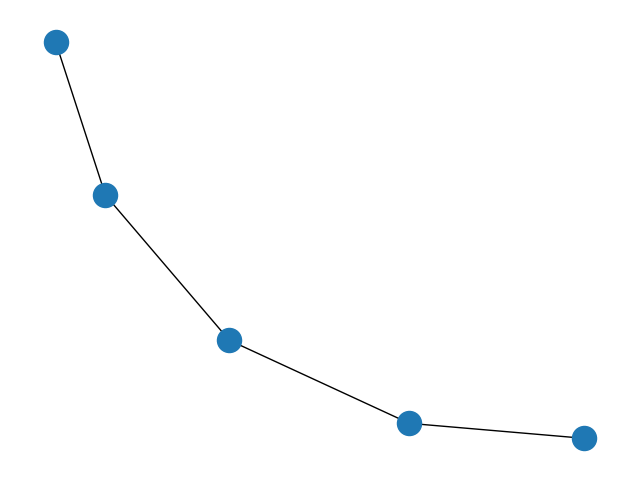
\includegraphics[width=\textwidth]{path/graph}
    \caption{Path graph}
    \end{subfigure}
\hfill
    \begin{subfigure}{0.32\textwidth}
    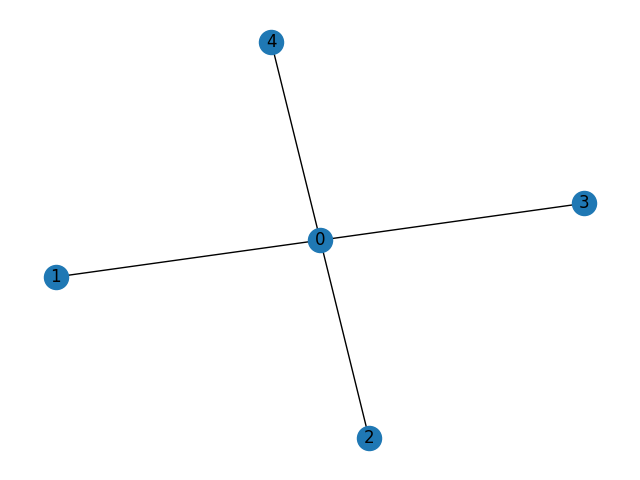
\includegraphics[width=\textwidth]{star/graph}
    \caption{Star graph}
    \end{subfigure}
\caption{Different graphs checked}
\label{Graphs}
\end{figure}

\bigskip
We have tested three different graphs represented in figure \ref{Graphs}:
\begin{itemize}
\item cycle graph
\item path graph
\item star graph
\end{itemize}

From these experiments we would expect that fewer epochs are needed in the case of a more connected graph such as the cycle than in the case of a less connected one such as the star graph.

\begin{figure}[H]
\centering
	\begin{subfigure}{0.49\textwidth}	
	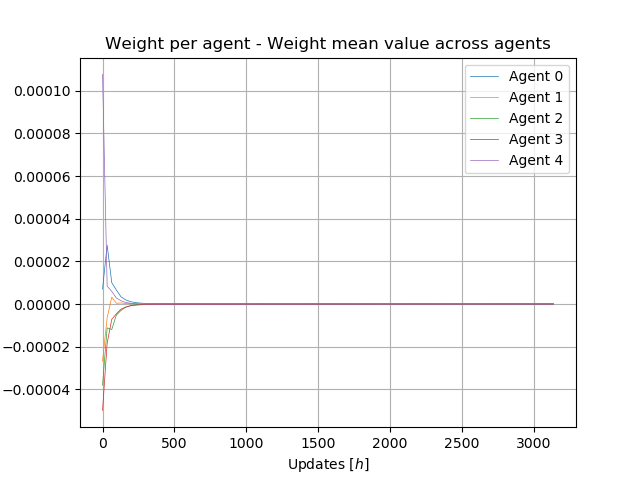
\includegraphics[width=\textwidth]{cycle/weight_100}
	\caption{Consensus error evolution}
	\end{subfigure}
\hfill
	\begin{subfigure}{0.49\textwidth}	
	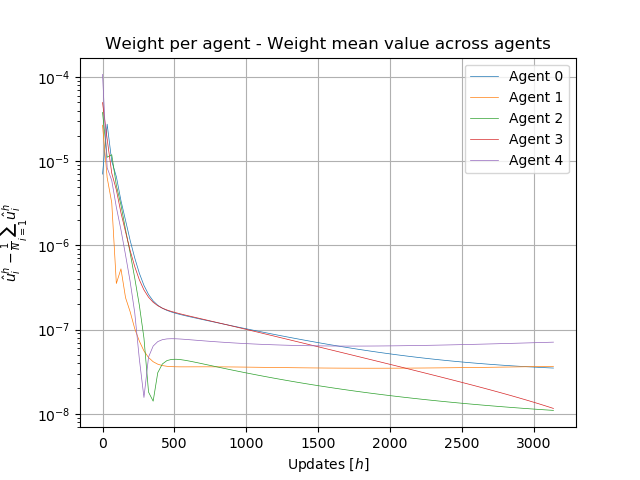
\includegraphics[width=\textwidth]{cycle/weight_100_log}
	\caption{Consensus error evolution in log-scale}
	\end{subfigure}
\caption{Evolution of a weight to consensus with \textbf{cycle} graph over 100 epochs}
\label{cycle_test}
\end{figure}

In fact, the cycle graph is the fastest to reach consensus as the nodes have all the same "connectivity" and the information travels smoothly. This is immediately reflected in figure \ref{cycle_test} where we see how the weights approach the average at approximately the same rate. Considering as a threshold value to say that the consensus is reached $10^{-7}$, in this training this value is reached in about $1000$ updates.

\begin{figure}[h]
\centering
	\begin{subfigure}{0.49\textwidth}	
	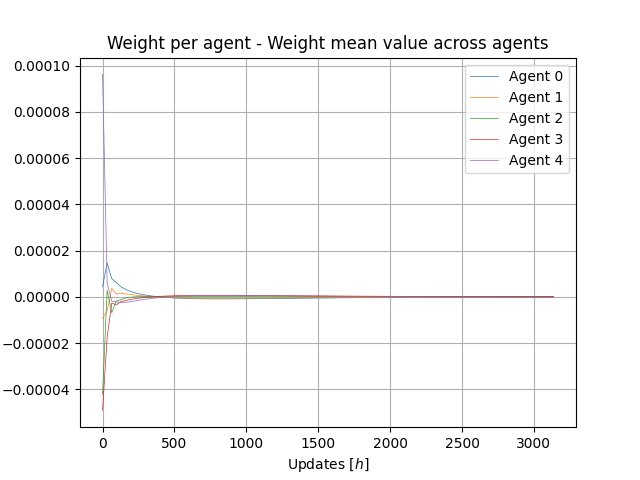
\includegraphics[width=\textwidth]{path/weight_100}
	\caption{Consensus error evolution}
	\end{subfigure}
\hfill
	\begin{subfigure}{0.49\textwidth}	
	\includegraphics[width=\textwidth]{/path/weight_100_log}
	\caption{Consensus error evolution in log-scale}
	\end{subfigure}
\caption{Evolution of a weight to consensus with \textbf{path} graph over 100 epochs}
\label{path_test}
\end{figure}

In case of the path graph, less connected than the cycle, the value of $10^{-7}$ requires more updates to be reached.


\begin{figure}[h]
\centering
	\begin{subfigure}{0.49\textwidth}	
	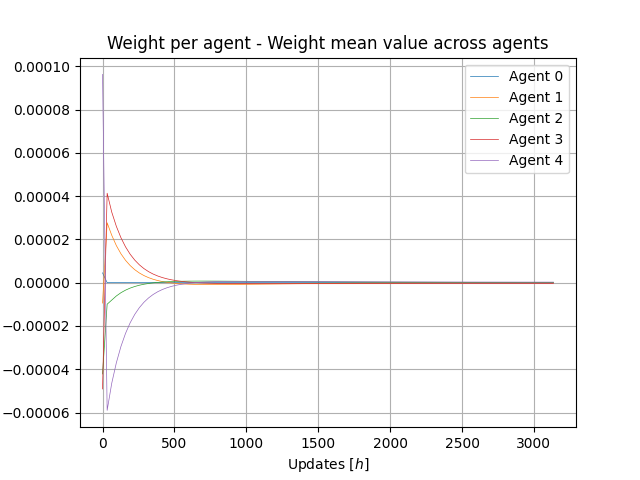
\includegraphics[width=\textwidth]{star/weight_100}
	\caption{Consensus error evolution}
	\end{subfigure}
\hfill
	\begin{subfigure}{0.49\textwidth}	
	\includegraphics[width=\textwidth]{star/weight_100_log}
	\caption{Consensus error evolution in log-scale}
	\end{subfigure}
\caption{Evolution of a weight to consensus with \textbf{star} graph over 100 epochs}
\label{star_test}
\end{figure}

Differently, in the figure \ref{star_test}, representing the star graph, we observe that the more connected node (the centre of the star, agent 0) approaches the average at a faster pace with respect to the less connected ones.

\section{Fourth test: diminishing stepsize}
Since the simulation requires a high computational time we have tried to run a simulation with a diminishing stepsize instead of a constant one. In this case we have chosen to start from a stepzise equal to $1e^{-1}$ that decreases linearly during the iterations up to a stepsize of $1e^{-6}$.
After $3092$ epochs the simulation stopped since we have introduced a stopping criterion on the decreasing rate of the gradient of the cost function: if in the last $500$ epochs, the gradient has diminished of a value smaller than $1e^{-5}$ the simulation stops.

\begin{figure}[h]
\centering
	\begin{subfigure}{0.49\textwidth}	
	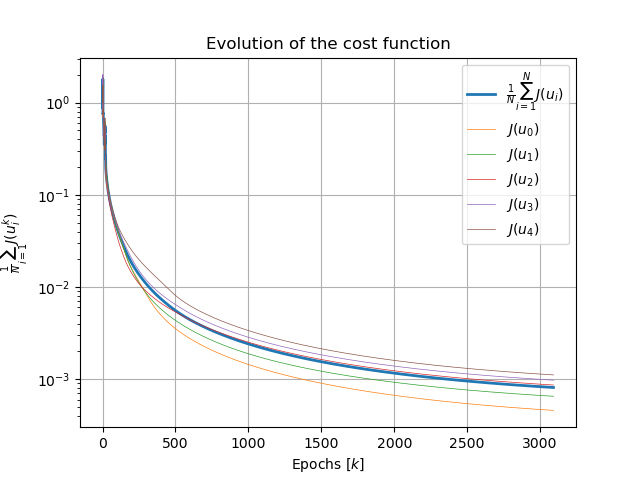
\includegraphics[width=\textwidth]{diminishing/J-log}
	\caption{Cost evolution in log-scale}
	\end{subfigure}
\hfill
	\begin{subfigure}{0.49\textwidth}	
	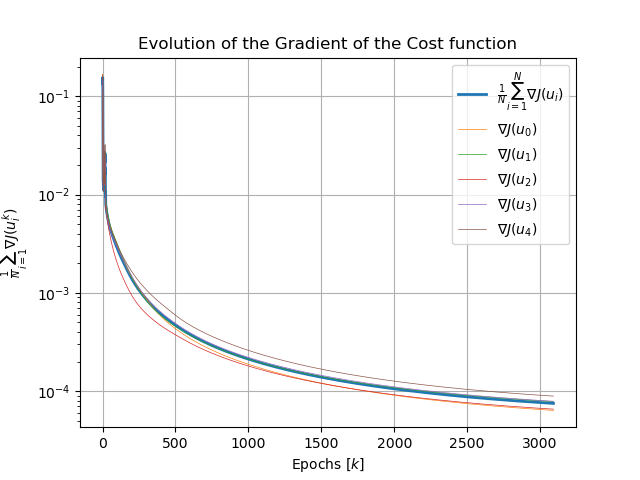
\includegraphics[width=\textwidth]{diminishing/norm_gradient_J}
	\caption{Gradient evolution in log-scale}
	\end{subfigure}
\caption{Evolution of the cost function and of the gradient.}
\label{diminish_cost_grad}
\end{figure}

This test has produced, as shown in figure \ref{diminish_cost_grad} very good results: the gradient reaches a value smaller than $1e^{-4}$, so the resulting weights will be very close to the optimum consensus value. 

\begin{figure}[h]
\centering
	\begin{subfigure}{0.49\textwidth}	
	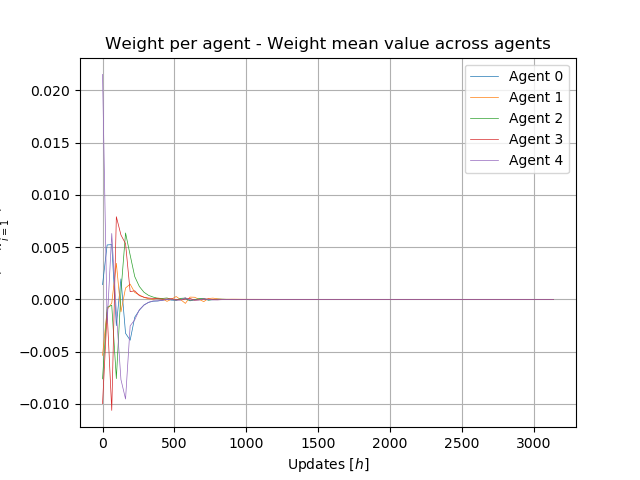
\includegraphics[width=\textwidth]{diminishing/weight_100}
	\caption{Consensus error evolution}
	\end{subfigure}
\hfill
	\begin{subfigure}{0.49\textwidth}	
	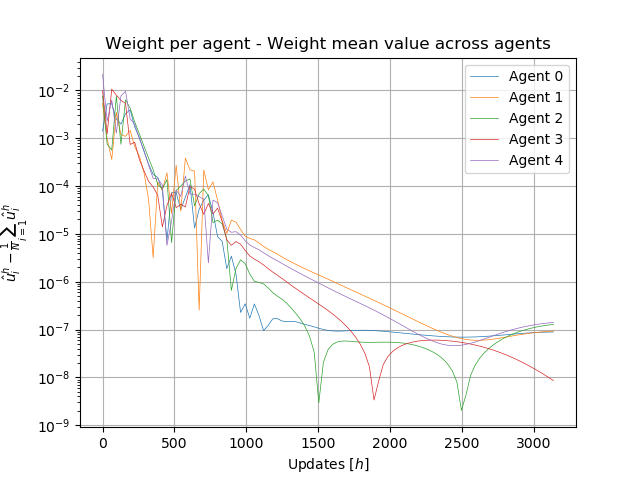
\includegraphics[width=\textwidth]{diminishing/weight_100_log}
	\caption{Consensus error evolution in log-scale}
	\end{subfigure}
\caption{Evolution of a weight to consensus with diminishing stepsize over 100 epochs}
\label{diminish_weights}
\end{figure}
\bigskip

Also, the results about consensus in \ref{diminish_weights} seems to be good but not so different with respect to the ones obtained with the constant stepsize. We could conclude that the stepsize does not influence so much the convergence rate to the consensus value.


\chapter{Formation Control} 
 In the second task we were asked to implement in ROS2 a discrete-time version of a \textbf{formation control law} for a team of $N$ robots.

\section{Distance-based formation}
The aim of the task was to obtain a desired geometric formation among a group of $N$ autonomous agents, by acting on the relative positions of agents.

\bigskip
The desired formation can be encoded in terms of an undirected graph, called \textit{formation graph}, whose set of vertices is indexed by the team agents $\mathcal{N} =\{ 1, \ldots, N\}$, and whose set of edges $E=\{(i,j) \in \mathcal{N} \times \mathcal{N} | \, j \in \mathcal{N}_i\}$ contains pairs of agents, where $\mathcal{N}_i$ are the neighbors of agent $i$. Each edge $(i,j) \in E$ is assigned a scalar parameter $d_{ij} = d_{ji} > 0$, representing the distance at which agents $i,j$ should converge to. 

An example could be a predefined formation with hexagon shape with the following \textit{distances matrix}:
\begin{equation}
d_{ij} =
\begin{bmatrix}
0 & l & 0 & d & h & l \\
l & 0 & l & 0 & d & 0 \\
0 & l & 0 & l & 0 & d \\
d & 0 & l & 0 & l & 0 \\
h & d & 0 & l & 0 & l \\
l & 0 & d & 0 & l & 0
\end{bmatrix}
\end{equation}
The desired distance value serve as reference value for the control law. The control law computes control signals for each agent based on its current position and the position of the neighboring agents, aiming to drive the agents towards the desired formation.
The neighbors of a certain agent $i$ can be extracted from the $i$-th row of the distances matrix, by taking the indexes of the elements with $d_{ij} > 0$.

By denoting the position of agent $i \in \{1, \cdots, N\}$ at time $t>0$ with $x_i(t) \in \mathbb{R}^3$, one way to approach distance-based formation control involves the usage of \textbf{potential functions}, similar to the following one:
\begin{equation}
V_{ij}(x)  = \frac{1}{4} \bigg( \lVert x_i - x_j \rVert^2 - d_{ij}^2 \bigg)^2
\label{Formation_potential}
\end{equation}

This kind of potential function represents the energy associated with the relative positions of the agents. By minimizing this potential function, the agents can achieve and maintain the desired formation, running as dynamics the opposite of the gradient of the potential function.
As a consequence, the control law we have implemented for each agent $i$ is the following:
\begin{equation}
\dot{x}_i(t) = f_i(x(t)) = - \sum_{j \in \mathcal{N}_i} \bigg( \lVert x_i - x_j \rVert^2 - d_{ij}^2 \bigg) (x_i - x_j )
\label{Dynamics_no_collision_avoidance}
\end{equation}

Since we were required to work in discrete time, we denote with $p_i^k \in \mathbb{R}^3$ the discretized version of $x_i(t)$ at iteration $k \in \mathbb{N}$ and, once we have computed the dynamic update for agent $i$ we discretize it with Euler formula in the following way:
\begin{equation}
p_i^{k+1} = p_i^{k} + \Delta f_i(p^k)
\end{equation}
where $\Delta > 0$ is the sampling period.

\section{ROS2 implementation}
The solution proposed in the previous section has been implemented in ROS2 environment with a code written in Python language.

\bigskip
By means of a launch file (named \texttt{formation\_control.launch.py}), we can generate the desired number of agents and give them the required information in order to accomplish the target formation. In particular, for each agent, the launch file generates a ROS2 node that executes the file named \texttt{the\_agent.py}. Each node gets the following main parameters from the launch file:
\begin{itemize}
\item id: a number from $0$ to $N-1$ associated with the agent's identity;
\item initial position, randomly generated;
\item distances: each agent gets only "its" row of the distances matrix. In this way it will be able to know who are its neighbors and the distances he has to keep from them in the desired configuration;
\item maximum number of dynamic updates.
\end{itemize}
This file manages the dynamic evolution of the agent and the communication with the other ones (the neighbors' ones). For what regards the communication, we have used a publisher-subscriber protocol implemented in ROS2: each node communicates its id, current iteration and position only to its neighbors. 
The communication between nodes is made by creating a topic for each agent in the network and letting the neighbors subscribe to the topic, so that they can access to the published information.

\bigskip
We have developed also a plotter agent (\texttt{the\_plotter.py}) that can read the actual positions of all the other agents in order to visualize the evolution of the trajectories of the whole formation.

For what regards the simulation and visualization of the team behaviour, we have used RViz.

\subsection{Results}
In the following we can see some results obtained during the simulation of the \texttt{formation\_control} package. 
We have tested several formation-shapes that involve different number of agents.


\begin{figure}[h]
\centering
	\begin{subfigure}{0.49\textwidth}	
	\centering
	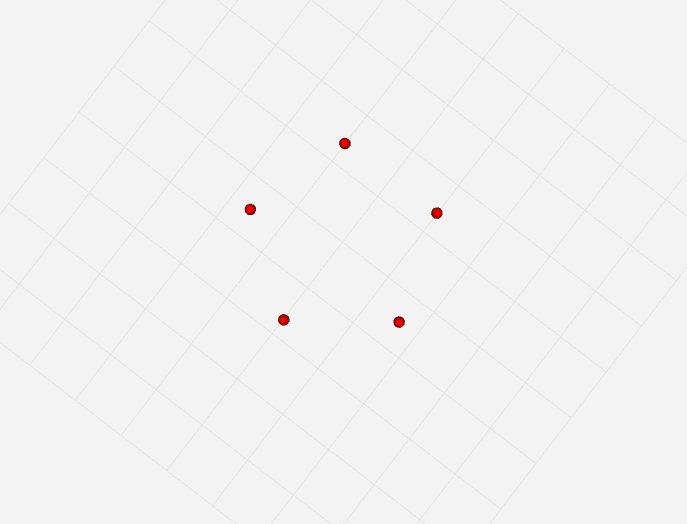
\includegraphics[width=0.9\textwidth]{pentagon_rviz.png}
	\caption{RViz visualization}
	\end{subfigure}
\hfill
	\begin{subfigure}{0.49\textwidth}	
	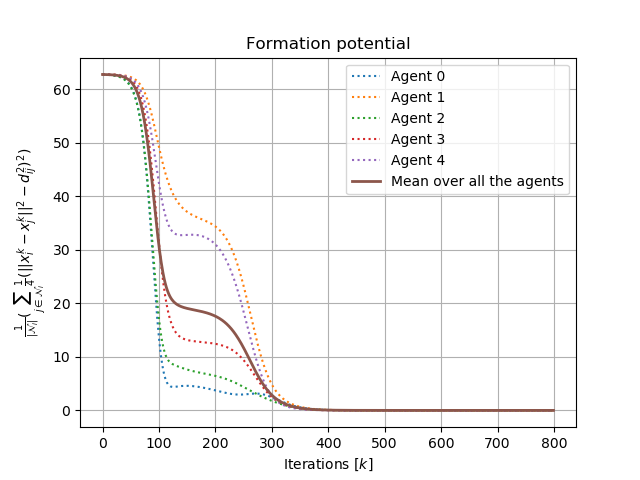
\includegraphics[width=\textwidth]{Formation_potential_pentagon.png}
	\caption{Formation potential plot}
	\end{subfigure}
\caption{Pentagon formation with $5$ agents}
\label{Pentagon}
\end{figure}

\begin{figure}
\centering
	\begin{subfigure}{0.49\textwidth}	
	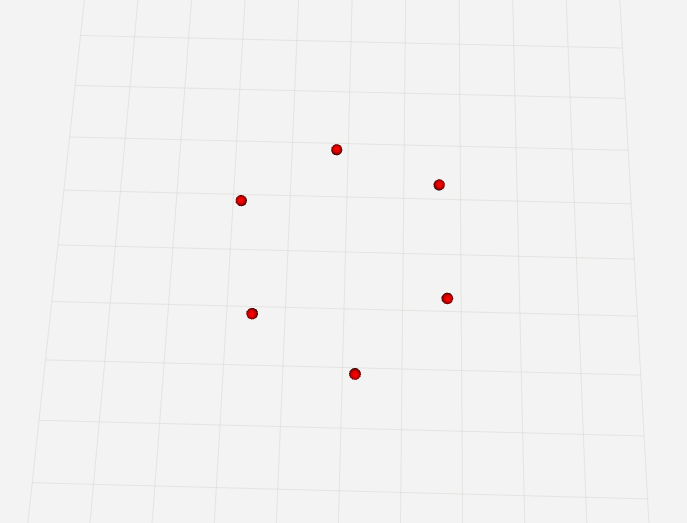
\includegraphics[width=0.9\textwidth]{hexagon_rviz.png}
	\caption{RViz visualization}
	\end{subfigure}
\hfill
	\begin{subfigure}{0.49\textwidth}	
	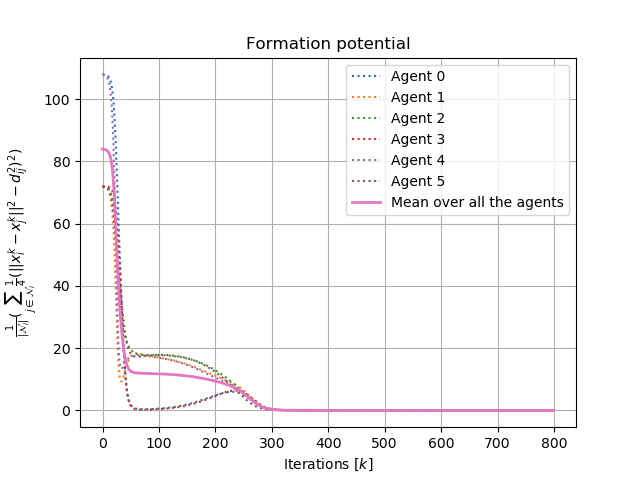
\includegraphics[width=\textwidth]{Formation_potential_hexagon.png}
	\caption{Formation potential plot}
	\end{subfigure}
\caption{Hexagon formation with $6$ agents}
\label{Hexagon}
\end{figure}

\begin{figure}
\centering
	\begin{subfigure}{0.49\textwidth}	
	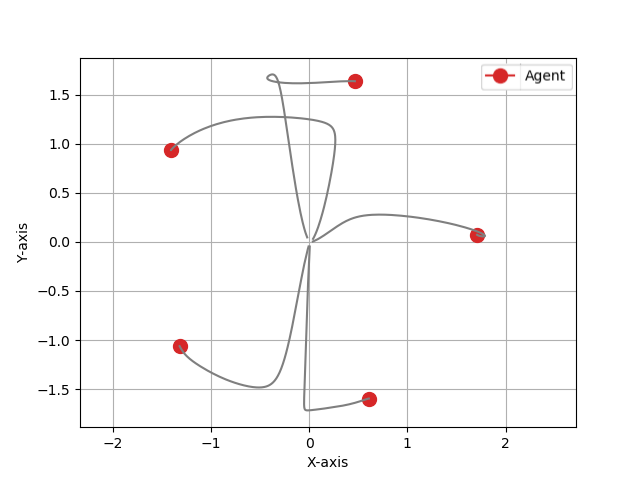
\includegraphics[width=\textwidth]{Pentagon_path.jpg}
	\caption{Paths for pentagon formation}
	\end{subfigure}
\hfill
	\begin{subfigure}{0.49\textwidth}	
	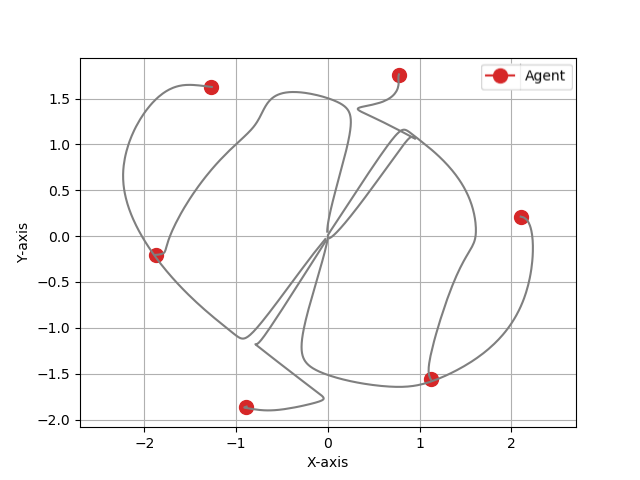
\includegraphics[width=\textwidth]{Hexagon_path.jpg}
	\caption{Paths for hexagon formation}
	\end{subfigure}
\caption{Paths followed by agents to reach formation}
\label{Paths}
\end{figure}

First of all we have tried 2D-formations like a pentagon and an hexagon, the results are represented respectively in figure \ref{Pentagon} and \ref{Hexagon}. We have initialized the agents positions randomly and close to zero for the $x$ and the $y$ dimensions, while $z$ position has been initialized equal to zero. Since our target formation is planar, the $z$ remains always equal to zero during the whole evolution.
We show both the final RViz visualization and the potential evolution during the iterations: for the single agents and for the whole formation. The potential diminishes along the iterations while the agents reach the desired configuration. 
For these formations we have also represented in figure \ref{Paths} the paths the single agents follow during the time evolution in order to accomplish the formation.

\begin{figure}
\centering
	\begin{subfigure}{0.49\textwidth}	
	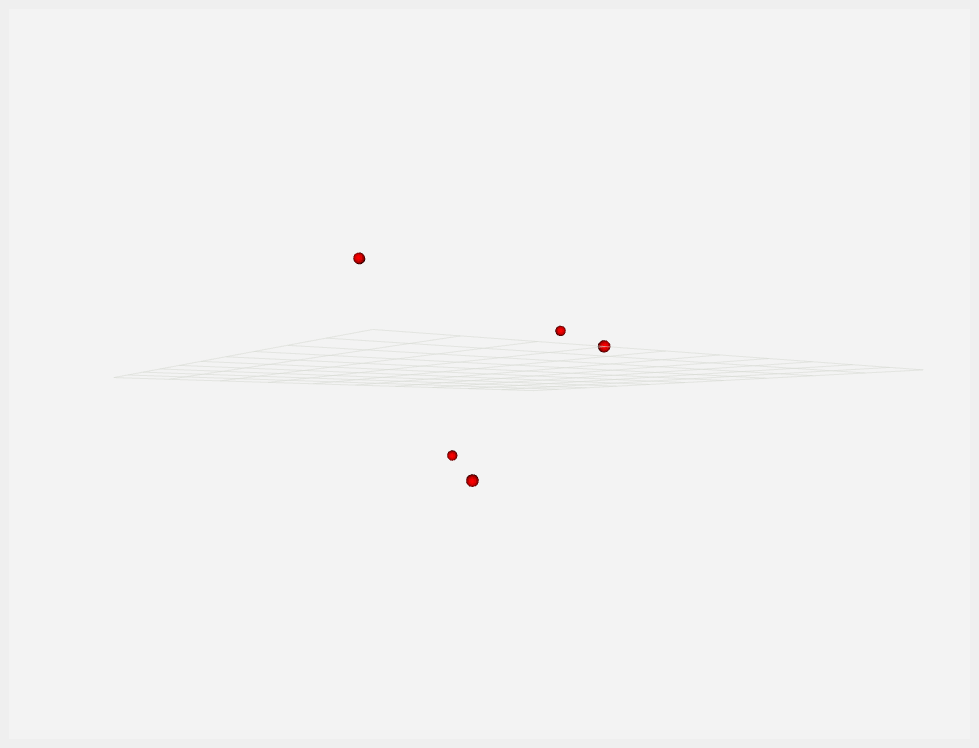
\includegraphics[width=0.9\textwidth]{Task-2.2_R-viz_No-Coll-Avoid_Piramid}
	\caption{RViz visualization}
	\end{subfigure}
\hfill
	\begin{subfigure}{0.49\textwidth}	
	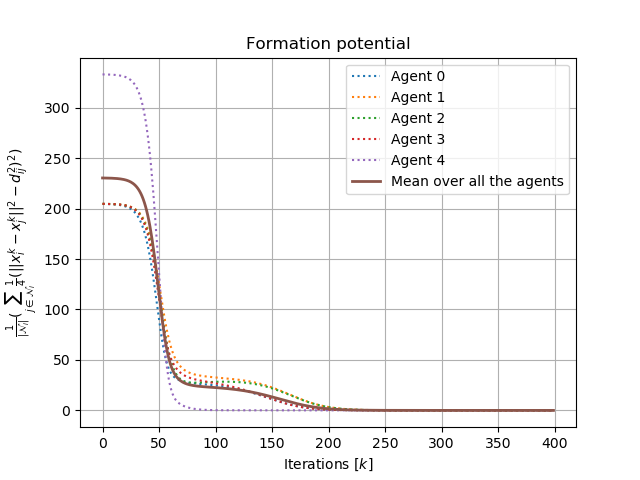
\includegraphics[width=\textwidth]{Formation_potential_piramid}
	\caption{Formation potential plot}
	\end{subfigure}
\caption{Square-based pyramid with $5$ agents}
\label{Piramid}
\end{figure}

After that, we have tried a 3D-formation, a square-based pyramid. In order to do that we have initialized all the $x$, $y$ and $z$ positions close to zero. In figure \ref{Piramid} we can see the results obtained with our simulation. The plane chosen by the "base-agents" changes from one simulation to the others since we do not have any constraint in this sense.


\section{Collision avoidance}
In formation control, the control laws typically consist of two components: attraction and repulsion. The attraction component pulls the agents towards their desired positions relative to their neighbors, while the repulsion component prevents collision by creating a repulsive force when the agents get too close to each other.

\begin{figure}[h]
\centering
	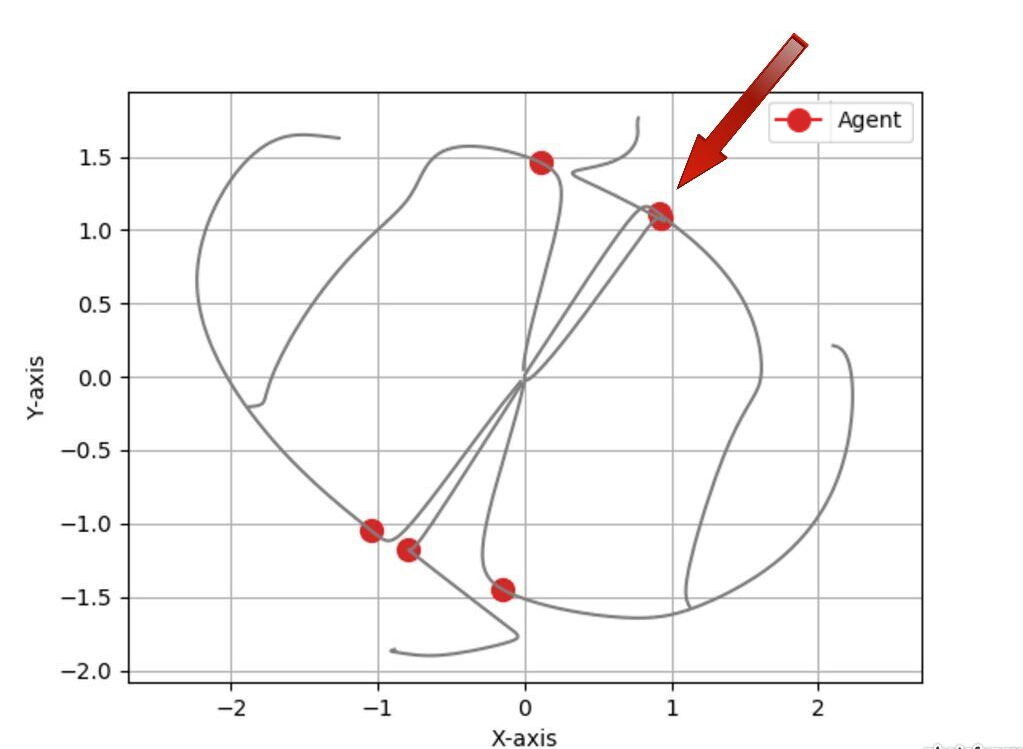
\includegraphics[scale=0.25]{Collision.jpg}
	\caption{Collision among two agents during hexagon formation (without collision avoidance term)}
	\label{Collision}
\end{figure}

The control law that models the agent's dynamics up to now, has just one component, the one linked to the formation potential, formula \ref{Formation_potential}, this was not enough in order to avoid collision among agents (as we can see in figure \ref{Collision}: two agents are in the same position at the same time). 

\bigskip
For this reason the \textbf{task 2.2} asked to introduce a second potential to avoid agent's collision. In order to do that the following proper barrier function has been used:
\begin{equation}
V_{ij}(x) = - \log( \lVert x_i - x_j \rVert ^2)
\label{Collision_barrier}
\end{equation}


As a result, the control law has a new term due to this potential that is the following one:
\begin{equation}
\dot{x}_i(t) = 2\sum_{j \in \mathcal{N}_i} \frac{(x_i-x_j)}{\big( \lVert x_i - x_j \rVert^2 \big)}
\end{equation}

And the total control law becomes:
\begin{equation}
\dot{x}_i(t) = - \Biggl( \sum_{j \in \mathcal{N}_i} \bigg( \lVert x_i - x_j \rVert^2 - d_{ij}^2 \bigg) (x_i - x_j ) - 2  \frac{(x_i-x_j)}{\big( \lVert x_i - x_j \rVert^2 \big)} \Biggr)
\label{Dynamics_with_collision_avoidance}
\end{equation}

\subsection{Results}
\begin{figure}[h]
\centering
	\begin{subfigure}{0.49\textwidth}	
	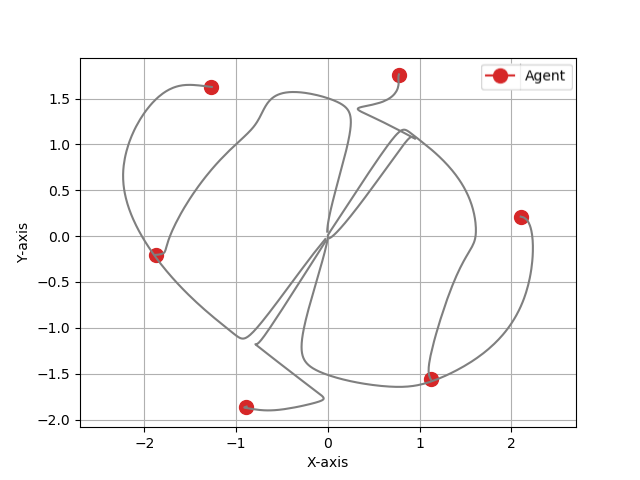
\includegraphics[width=\textwidth]{Hexagon_path.jpg}
	\caption{Path followed by agents without collision avoidance term}
	\end{subfigure}
\hfill
	\begin{subfigure}{0.49\textwidth}	
	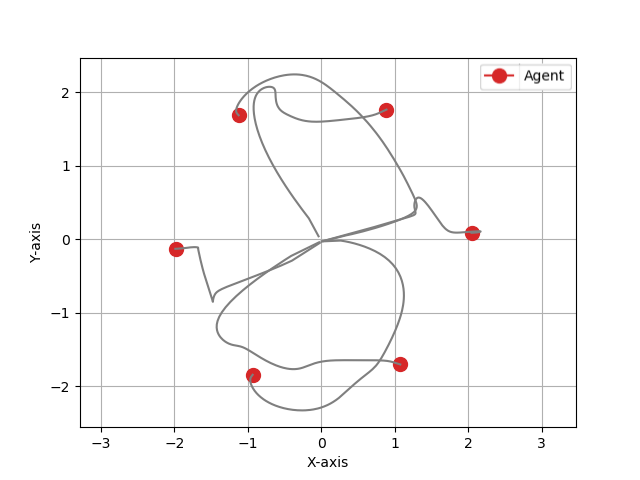
\includegraphics[width=\textwidth]{Hexagon_path_collision.jpg}
	\caption{Path followed by agents with collision avoidance term}
	\end{subfigure}
\caption{Comparison among paths with and without collision avoidance term}
\label{Paths_comparison}
\end{figure}

In figure \ref{Paths_comparison} we can see the different shape of the paths followed by the agents in order to reach the same hexagon formation. The plot on the left shows the paths due to the dynamic evolution expressed in formula \ref{Dynamics_no_collision_avoidance} (the one without the collision avoidance term), while the plot on the right shows the behaviour due to the introduction of the collision avoidance term (formula \ref{Dynamics_with_collision_avoidance}).

\begin{figure}[h]
\centering
	\begin{subfigure}{0.49\textwidth}	
	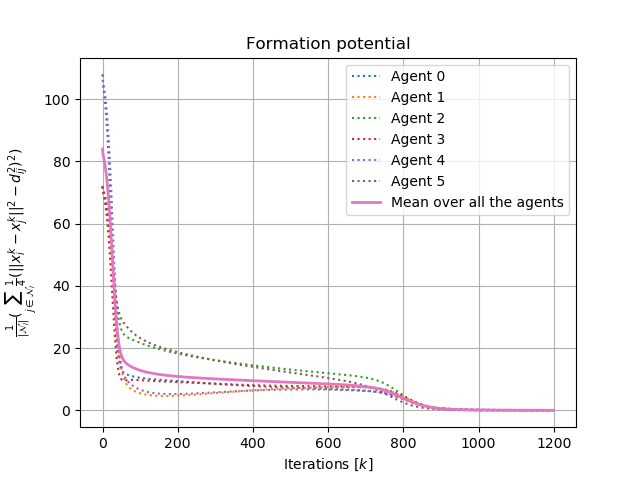
\includegraphics[scale=0.42]{Task-2.2_Formation-p_Yes-Coll-Avoid_Hexagon}
	\caption{Formation potential (attraction) term}
	\end{subfigure}
\hfill
	\begin{subfigure}{0.49\textwidth}	
	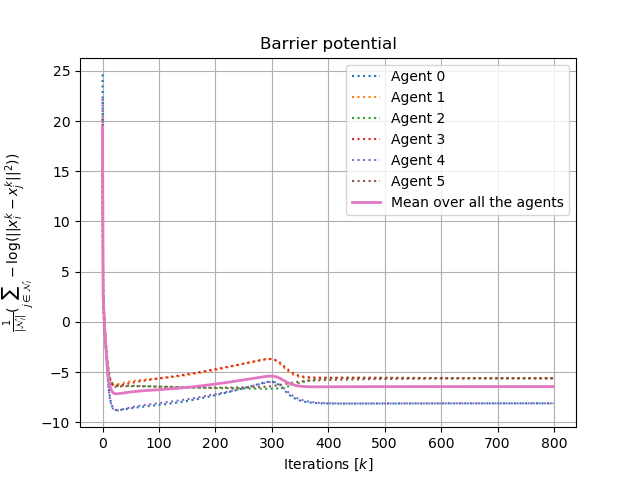
\includegraphics[scale=0.42]{Barrier_potential_hexagon_collision.png}
	\caption{Barrier potential (repulsion), collision avoidance term}
	\end{subfigure}
\caption{Potential contribution in hexagon formation with collision avoidance}
\label{Potentials_with_collision}
\end{figure}

In figure \ref{Potentials_with_collision} we can see the evolution of the two contributions of the overall potential function. The formation potential, the attractive one that pulls the agents toward the desired formation, diminishes but we can see a "flat area" when the agents go too close to some neighbors. Accordingly, the barrier potential that repels the agents from neighbors, has a peak.

\section{Moving formation and leaders control}
At this point robots are partitioned in two groups, namely leaders and followers. The objective of \textbf{task 2.3} is to control the translation and/or the rotation of the formation (by giving proper inputs to the leaders) while maintaining the chosen pattern.
Distance constrains  are invariant to both translation and rotation of the formation, so the distance-based approach can be applied to realize translational and rotational formation maneuvers. 

We have modified the \texttt{formation\_control.launch.py} in order to pass to the \texttt{the\_agent.py} file the information about their identity (leader or follower) and about the motion the leaders have to accomplish.

\begin{figure}[h]
\centering
	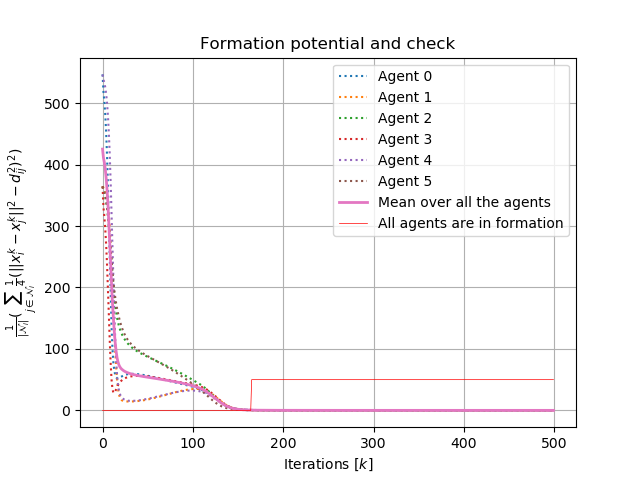
\includegraphics[scale=0.6]{Task-2.3_Formation-p_Linear-trj_Hexagon}
	\caption{Check on the formation accomplishment}
	\label{Check}
\end{figure}

\bigskip
We use the \texttt{the\_plotter} agent as a "supervisor" that tells all the agents when the target formation has been reached. Once all the agents are in formation the leaders start moving. As a trigger condition the supervisor checks when the potentials' derivatives of all the agents are smaller than a certain threshold. At this moment, he notifies all the agents the formation has been reached and so, the leaders can start moving. This threshold value depends on the formation shape we chose. In figure \ref{Check} the red line represents this notification criterion.

\bigskip
From this moment on, the dynamic evolution changes: the followers continue with the same motion, trying to maintain the formation, while the leader's dynamic has two contributions, the formation one and the motion we have decided them to follow. Both have also the collision avoidance term.

\begin{figure}[h]
\centering
	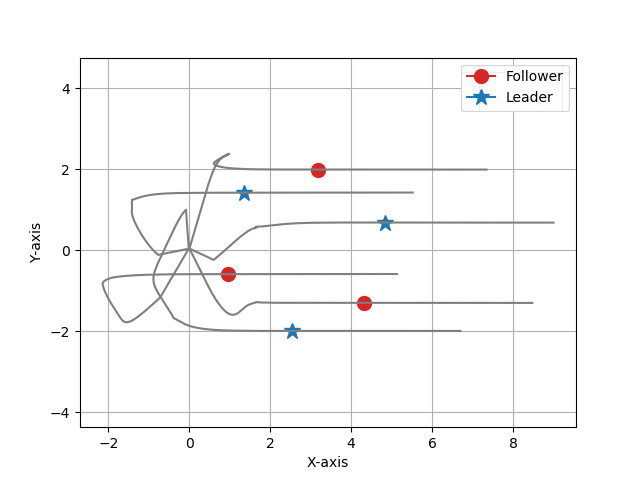
\includegraphics[scale=0.4]{Moving_hexagon_formation_linear.jpg}
	\caption{Motion of the formation along the $x$-axis}
	\label{Formation_motion_lin}
\end{figure}

Figure \ref{Formation_motion_lin} represents the motion of the formation along the $x$-axis due to a constant input assigned to leaders' dynamic. The leaders are represented as the blue stars.

\begin{figure}[h]
\centering
	\begin{subfigure}{0.49\textwidth}	
	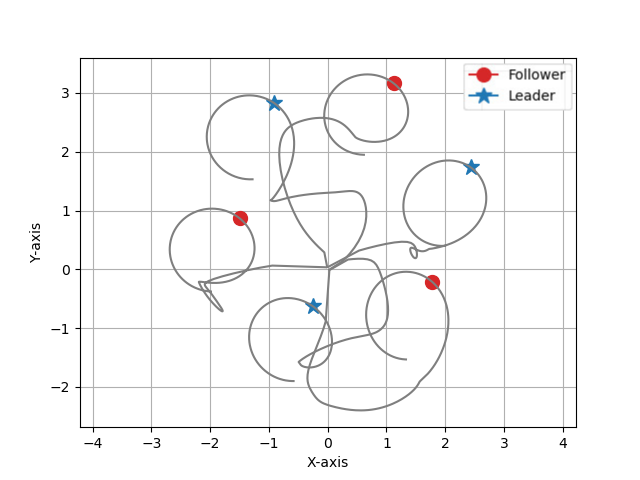
\includegraphics[width=\textwidth]{Moving_hexagon_formation_circle_r_2.jpg}
	\caption{Motion along a circle of radius $2$}
	\end{subfigure}
\hfill
	\begin{subfigure}{0.49\textwidth}	
	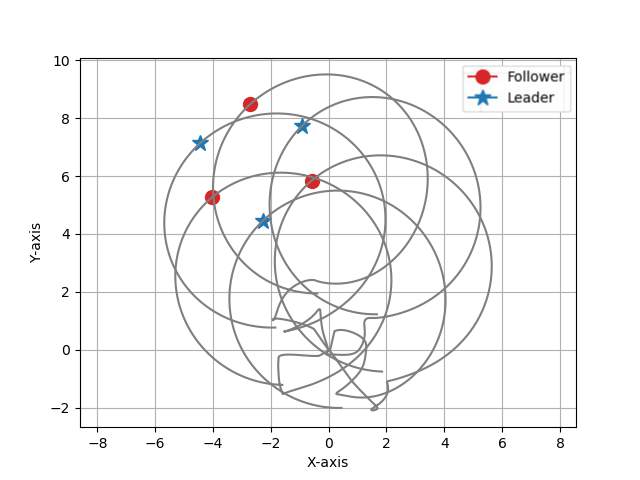
\includegraphics[width=\textwidth]{Moving_hexagon_formation_circle_r_5.jpg}
	\caption{Motion along a circle of radius $5$}
	\end{subfigure}
\caption{Motion of the formation along a circular path}
\label{Formation_motion_circle}
\end{figure}

\bigskip
We have also tried to give the leaders a proper input in order to accomplish a circular motion during the number of iterations given. In figure \ref{Formation_motion_circle} we can see the motion of the hexagon formation: in the left plot we have given as input a radius equal to $2$ while in the right one, the radius is equal to $5$.



\section{Obstacle avoidance}
\textbf{Task 2.4} asked for us to introduce obstacle avoidance in the formation dynamics (\texttt{formation\_control} package). Obstacle avoidance in formation control refers to the ability of a group of $N$ coordinated agents to navigate through an environment while maintaining a desired formation and avoiding collision with fixed or moving obstacles. 

In order to accomplish this task, we have created a certain number of fixed obstacles as ROS2 nodes. The obstacles get their position from the launch file and communicate it to the follower agents. 
In \texttt{the\_agent.py} we still have two dynamics: the leaders move according to the assigned input while the followers move according to the formation and trying to avoid obstacles. For this reason we have introduced in the dynamics a potential in order to avoid obstacles:
\begin{equation}
V_{ih}(x) = - \log( \lVert x_i - x_h\rVert ^2)
\label{Obstacles_barrier}
\end{equation}
where $x_h$ denotes the position of the obstacles.

\bigskip
In the following simulation we give to the leaders of the formation a target position (indicated in the plot with the yellow x symbol) "on top of" the obstacles: to reach it the formation has to pass inside the window left by the obstacles. 
The target position is assigned to the leaders in this way: when the formation in reached, each leader computes its target position as in the following:
\begin{equation}
x_{i,tar} = x_i(\bar{t}) + h_y, \text{     $i$ are leaders}
\end{equation}
where $\bar{t}$ is the time instant in which the formation is reached, and $h_y$ is a proper distance (in this case along $y$ direction). In our simulation we chose $h_y = 7$ in order to make the formation move towards the obstacles.

\bigskip
In order to steer the leaders, and as a consequence the whole formation toward the target position, we have used the following proportional controller:
\begin{equation}
\dot{x}_i(t) = k\cdot (x_{i,tar} - x_i(t)), \text{     $i$ are leaders}
\end{equation}
where $k$ is a proper proportional gain.

\begin{figure}[h]
\centering
	\begin{subfigure}{0.5\textwidth}	
	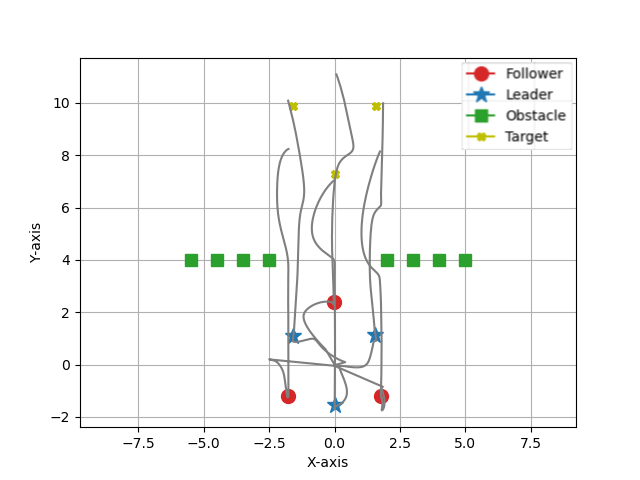
\includegraphics[width=\textwidth]{Hexagon_obstacle_Initial.jpg}
	\caption{Agents have reached the target formation}
	\end{subfigure}
\vfill
	\begin{subfigure}{0.5\textwidth}	
	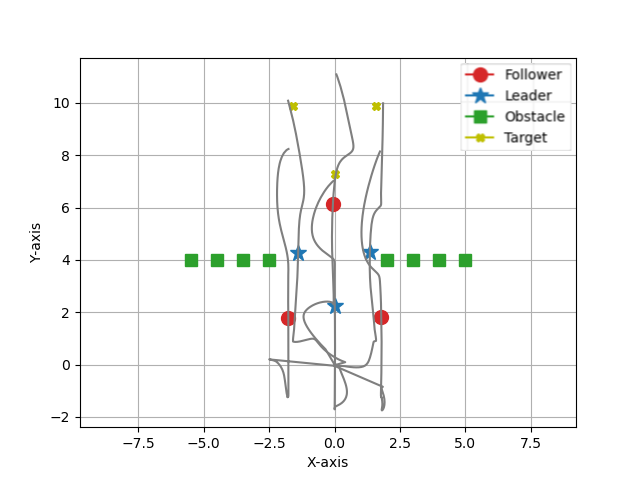
\includegraphics[width=\textwidth]{Hexagon_obstacle.jpg}
	\caption{Motion of formation to pass in between obstacles}
	\end{subfigure}
\vfill
	\begin{subfigure}{0.5\textwidth}	
	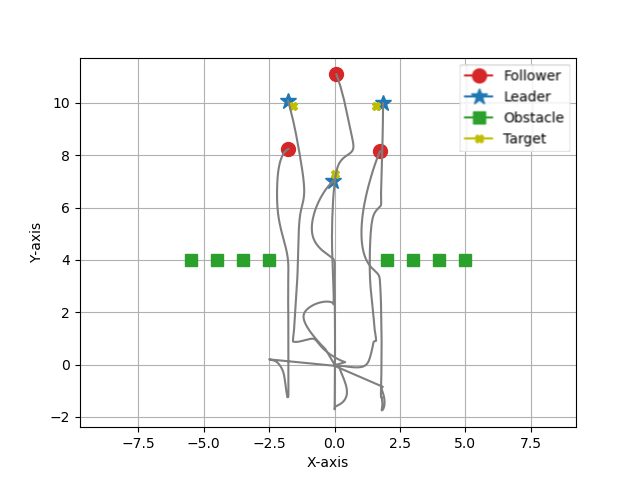
\includegraphics[width=\textwidth]{Hexagon_obstacle_target.jpg}
	\caption{Formation that reaches target position}
	\end{subfigure}
\caption{Obstacle avoidance and motion to target position}
\label{obstacle}
\end{figure}

As a consequence the control laws implemented in this task are the following:
\begin{equation}
\scriptsize
\dot{x}_i(t) = - \Biggl( \sum_{j \in \mathcal{N}_i} \bigg( \lVert x_i - x_j \rVert^2 - d_{ij}^2 \bigg) (x_i - x_j ) - 2  \frac{(x_i-x_j)}{\big( \lVert x_i - x_j \rVert^2 \big)} \Biggr) + 2  \sum_{h \in \mathcal{H}} \frac{(x_i-x_h)}{\big( \lVert x_i - x_h \rVert^2 \big)}  
\label{follower}
\end{equation}

\begin{equation}
\scriptsize
\dot{x}_i(t) = - \Biggl( \sum_{j \in \mathcal{N}_i} \bigg( \lVert x_i - x_j \rVert^2 - d_{ij}^2 \bigg) (x_i - x_j ) - 2  \frac{(x_i-x_j)}{\big( \lVert x_i - x_j \rVert^2 \big)} \Biggr) + k\cdot (x_{i,tar} - x_i)
\label{leaders}
\end{equation}
the \ref{follower} for the followers (i.e. $i \in \{1, \ldots, N_f\}$) and \ref{leaders} for the leaders (i.e. $i \in \{N_f+1, \ldots, N\}$), where $\mathcal{H}$ is the set of obstacles in the simulation.

\bigskip
In figure \ref{obstacle} we have represented three crucial points of the simulation. The first, \ref{obstacle}(a) represents the moment in which the formation in reached and leaders start moving toward the target. The second, \ref{obstacle}(b) represents the moment in which the formation is moving in between the window left by the obstacles: the shape of the hexagon is a bit distorted in order to allow the motion. The third, \ref{obstacle}(c), shows the moment in which the leaders reach their targets: at this point the formation has its right shape again.




%%%%%%%%%% Conclusions %%%%%%%%%%
\chapter*{Conclusions}
\addcontentsline{toc}{chapter}{Conclusions} 
In the \textbf{First task} we explored a distributed optimization framework where each individual agent possesses limited knowledge of the global optimization problem. To tackle the classification problem, agents rely solely on local computations and communication with their neighboring agents, without the involvement of a central unit. In order to solve this problem, we have implemented a Gradient Tracking algorithm. 
We have obtained good results both in terms of consensus and accuracy of the classification. 

A possible future development could be to train our neural network system in a truly distributed manner, with each network running on a separate processor, establishing a wired or wireless connection between devices. This would allow us to properly evaluate the benefits associated with distributed implementation.

\bigskip
In the \textbf{Second task} we have seen the power of a ROS2 implementation of formation control of network of N robotic agent, by applying a distance-based control law, and by allowing only local communication with neighbors. We have also seen how the agents are able to follow a predefined trajectory maintaining the formation very well.
Then, we explored the possibility of introducing obstacle and collision avoidance between agents and it seems to work very well. 

Future additional developments could be to try the formation control according to a bearing-based control technique in such a way to have also scale invariance in addition to translation and rotation one.

%%%%%%%%%% Bibliography %%%%%%%%%%%

%\bibliographystyle{sample}
%\bibliography{references}{}
%\addcontentsline{toc}{chapter}{Bibliography}


%%%%%%%%%%%%%%%%%%%%%%%%%%%%%%%%%%%%%%

\end{document}
